\documentclass[12pt]{exam}
\usepackage[phy]{template-for-exam}
\usepackage{pgfplots}
\pgfplotsset{
  compat=1.18,
  width=6cm,
  posgraph/.append style={
    axis y line = left,
    axis x line = center,
    axis line style = ultra thick,
    xlabel={\bf time},
    ylabel={\bf displacement},
    ymin=0,
    ymax=9,
    xmin=0,
    xmax=3,
    xtick=\empty,
    ytick=\empty,
  },
  regplot/.append style={smooth, domain=0:2.6},
  smallgraph/.append style={
    width=4.6cm,
    xlabel={\small time},
    ylabel={\small displacement},
    },
}
\usepackage{multicol}
\usepackage{graphicx}


\title{Motion \#4}
\author{Rohrbach}


\begin{document}
\maketitle

\begin{questions}

\question
  One of the following objects is moving forward.  The 
  other is moving backward.  Which is which?  Explain!!

  \begin{multicols}{2}

    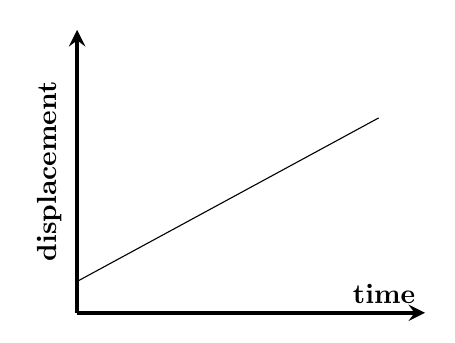
\begin{tikzpicture}
      \begin{axis}[posgraph]
        \addplot[regplot]{2*x+1};
      \end{axis}
    \end{tikzpicture}
    
    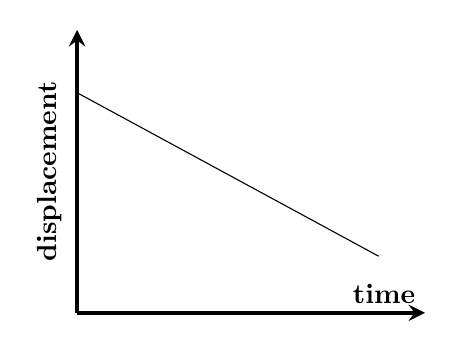
\begin{tikzpicture}
      \begin{axis}[posgraph]
        \addplot[regplot]{-2*x+7};
      \end{axis}
    \end{tikzpicture}

  \end{multicols}

\question
  We found out in the lab that the slope of the 
  displacement graph gives you the velocity.  Use 
  the concept of slope to explain why this object is 
  speeding up.

  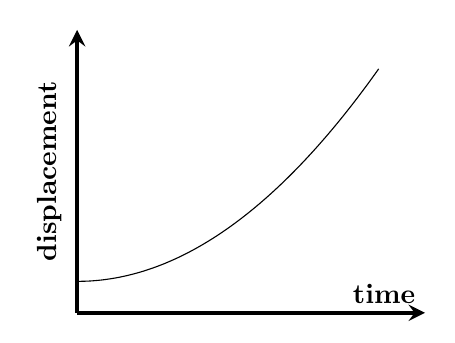
\begin{tikzpicture}
    \begin{axis}[posgraph]
      \addplot[regplot]{x^2+1};
    \end{axis}
  \end{tikzpicture}

\question
  Sketch the graph of an object that is moving forward 
  and slowing down.  Explain!!

  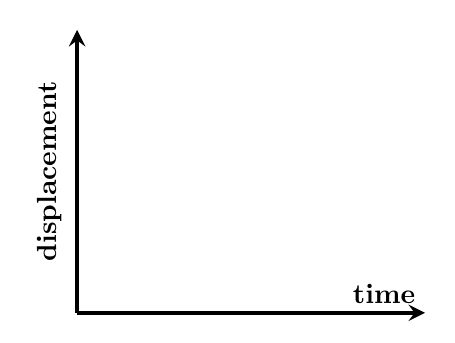
\begin{tikzpicture}
    \begin{axis}[posgraph]
    \end{axis}
  \end{tikzpicture}

\question
  For each of the following graphs, it is sufficient 
  to simply say whether the object is moving {\bf forward} 
  or {\bf backward} and whether it is {\bf speeding up}, 
  {\bf slowing down}, or {\bf maintaining a constant speed}. 


    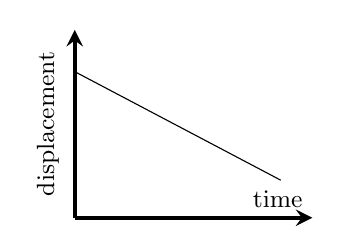
\begin{tikzpicture}
      \begin{axis}[posgraph,smallgraph]
        \addplot[regplot]{-2*x+7};
      \end{axis}
    \end{tikzpicture}
    %
    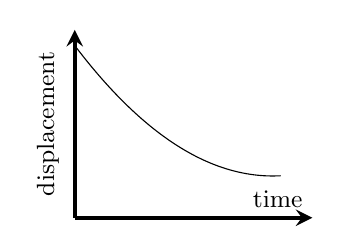
\begin{tikzpicture}
      \begin{axis}[posgraph,smallgraph]
        \addplot[regplot]{1*(x-2.5)^2+2};
      \end{axis}
    \end{tikzpicture}
    %
    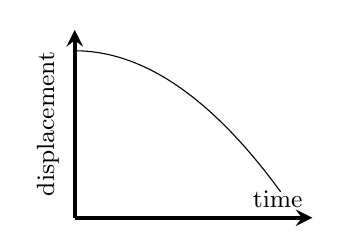
\begin{tikzpicture}
      \begin{axis}[posgraph,smallgraph]
        \addplot[regplot]{-1*x^2+8};
      \end{axis}
    \end{tikzpicture}
    %
    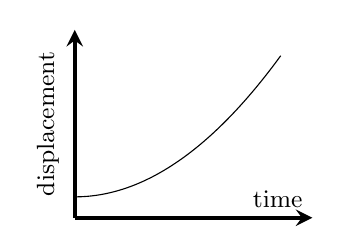
\begin{tikzpicture}
      \begin{axis}[posgraph,smallgraph]
        \addplot[regplot]{x^2+1};
      \end{axis}
    \end{tikzpicture}

\pagebreak

\question
  A graph of the motion of a tram at the airport 
  is shown below.  What is the tram’s velocity?

  
  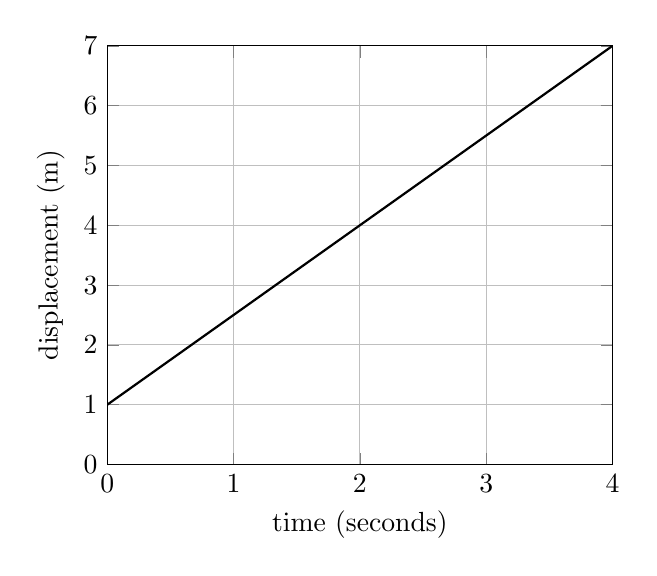
\begin{tikzpicture}
    \begin{axis}[
      axis y line = box,
      axis x line = box,
      axis y line shift = 0,
      axis line style = thin,
      xlabel={time (seconds)},
      ylabel={displacement (m)},
      ymin=0,
      ymax=7,
      xmin=0,
      xmax=4,
      grid=both,
      xtick = {0,...,5},
      ytick = {0,...,9},
      width=8cm
    ]
      \addplot[thick]{1.5*x+1};
    \end{axis}
  \end{tikzpicture}

\question
  Consider the motion maps of the cars below.  All of the
  cars are moving forward.
  
  \begin{center}
    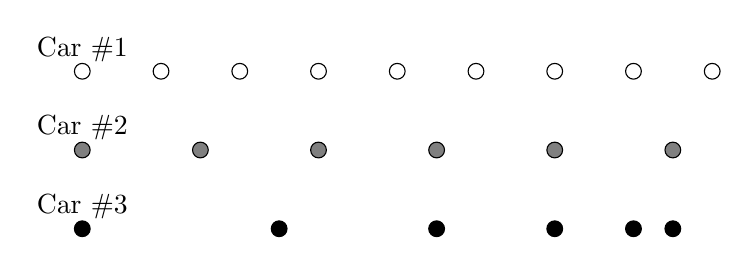
\begin{tikzpicture}
      \def\carone{1}
      \def\cartwo{1.5}
      \begin{scope}
        \filldraw[fill=white] (0,3) 
          node[anchor=south]{Car \#1}
          circle (0.1);
        \foreach \x in {1,...,8} {
          \filldraw[fill=white] (\x*\carone,3) circle (0.1);
        }
      \end{scope}
      \begin{scope}
        \filldraw[fill=gray] (0,2) 
          node[anchor=south]{Car \#2}
          circle (0.1);
        \foreach \x in {1,...,5} {
          \filldraw[fill=gray] (\x*\cartwo,2) circle (0.1);
        }
      \end{scope}
      \begin{scope}
        \filldraw[fill=black] (0,1) 
          node[anchor=south]{Car \#3}
          circle (0.1);
        \foreach \x in {2.5,4.5,6,7,7.5} {
          \filldraw[fill=black] (\x,1) circle (0.1);
        }
      \end{scope}
    \end{tikzpicture}
  \end{center}

  \begin{parts}

    \part
      Compare and contrast the motion of Cars \#1 and \#2.
      \vspace{\stretch{1}}

    \part
      What is happening to Car \#3?
      \vspace{\stretch{1}}

    \part
      Sketch graphs of the motion of each of the cars.
      \begin{multicols}{3}

        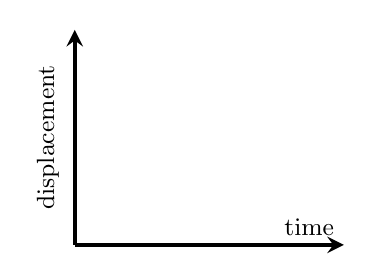
\begin{tikzpicture}
          \begin{axis}[posgraph,smallgraph,width=5cm]
          \end{axis}
        \end{tikzpicture}

        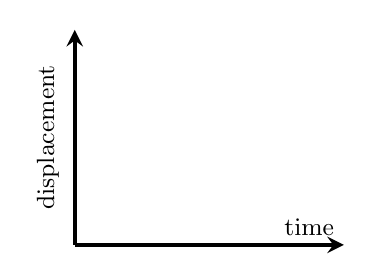
\begin{tikzpicture}
          \begin{axis}[posgraph,smallgraph,width=5cm]
          \end{axis}
        \end{tikzpicture}

        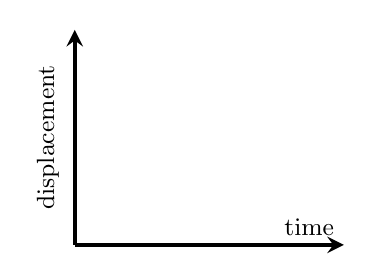
\begin{tikzpicture}
          \begin{axis}[posgraph,smallgraph,width=5cm]
          \end{axis}
        \end{tikzpicture}


      \end{multicols}


  \end{parts}

\end{questions}
\end{document}